\chapter{Introduction} \index{Introduction@\emph{Introduction}}%

\section*{Preface}
\addcontentsline{toc}{section}{Preface}%

    Heart valves play a critical role of preventing back flow during cardiac operations. They are designed to withstand the demanding mechanical environment of the heart while maintaining an optimal state for over 3 billion cycles. When they can no longer function properly due to fatigue, diseases or trauma, and when surgical repair is not an option, surgical replacement using bioprosthetic heart valves is often the best choice. This introductory chapter focus on the current state of heart valve replacements and design, and methods for improving the durability of these devices. First, an overview of the structure and functions of heart valves is provided. Then the current state of heart valve repair and replacement is summarized, followed by the current state of bioprosthetic valve design and fabrication as well as their durability and limitations. Finally, the causes and mechanisms of bioprosthetic heart valve failure is discussed, and we outline the motivation, rationale and aims of this dissertation, on how constitutive modeling and simulations can be used to better understand bioprosthetic heart valve failure and facilitate the improvement of bioprosthetic heart valve design. 


\section{Introduction and Background}

    Cardiovascular diseases remain the leading cause of death (31.8\% of all deaths) in U.S., costing 320.1 billion each year \cite{mozaffarian_heart_2015}. One significant area that need improvements is heart valve replacement and repair procedures such as aortic valve repair using bioprosthetic heart valves (BHVs), where the mortality has not seen any major improvements since 1985 – the rate of survival after 10 years still remains only 29.7\%. Soft-tissue-derived exogenously cross-linked (EXL) biomaterials, which has only existed since the beginning of 1970s, is the dominant choice due to advantages in immunogenicity and flow dynamics over their mechanical counter parts \cite{starr_artificial_2007}. However, our understanding of these materials and of the mechanisms of their failure is still incomplete. As such, current design and development is very empirical in nature – depending on trial and error, extrapolation from accelerated wear test and long periods of clinical testing. The need for better BHV designs is further accelerated by the emergence of percutaneous devices such as the transcather aortic valve replacement (TAVR) \cite{bonow_accaha_2006}\cite{guidoin_marvel_2010}. TAVRs are an attractive alternative to open heart surgeries, especially for people at high surgical risk, as well as youths who may require multiple surgical replacements over their life-time. However, they are more often associated with peri-valvular regurgitation and is currently lacking in long-term data pertaining to their durability \cite{guidoin_marvel_2010}. Existing TAVR data suggest only 2-year mortality rate of 33.9\% \cite{kodali_two_2012} in general and 68\% for aortic valve stenosis \cite{makkar_transcatheter_2012}. Much of the existing challenges is associated with the necessary compact folded delivery system, which places additional constraints on their geometrical design and mechanical properties. It is clear that there is a strong need for a better understanding of the mechanism associated with their failure and frameworks for predicting the long-term failure of these devices.
        
    

    
    
    
    
    
    





\subsection{Multi-scale structure of heart valves}

    To fully understand the functional properties of heart valves, multi-scale approaches are needed (Fig. \ref{fig:multiscalevalve}) \cite{salma_heart_2016}. This complex hierarchical structure is what lends to seamless heart valve performance under highly dynamic loading conditions. Heart valves have evolved to have multi-layered leaflet structures. The aortic valve, for example, consists of three histologically distinct layers, whereas the mitral valve has four (Fig. \ref{fig:valvelayers}). The fibrosa layer, which is located on the ventricular side of atrioventricular valves and the atrial side of semilunar valves, is composed of circumferentially aligned collagen fibers that provide the leaflets with the necessary tensile strength to open and transmit forces during coaptation while closed. The spongiosa layer is situated adjacent to the fibrosa and though it contains some collagen, its main constituents are the hydrophilic glycosaminoglycans and proteoglycans, which give the valve its compressive properties and allow it to absorb high forces during coaptation. The ventricularis and atrialis are the layers that are adjacent to blood flow in atrioventricular valvesand semilunar valves, respectively. These layers are rich in radially oriented elastin fibers and facilitate the closure movement by extending the valve leaflet as it opens and recoils when it closes. The annulus and chordae tendineae of the atrioventricular valves and the connection between the leaflets and the surrounding myocardium in the semilunar valves provide additional support. 


    Each layer contains varying amounts of collagen, glycosaminoglycan (GAG), and elastin \cite{carruthers_gene_2012}. The fibrosa layer, facing the outflow surface, consists primarily of a dense network of highly aligned type 1 collagen fibers and contributes to about 45\% of the valve thickness. The central spongiosa layer, approximately 30\% of the leaflet thickness is rich in glycosaminoglycans and water \cite{carruthers_gene_2012}. The ventricularis layer, the remaining 25\% of the leaflet faces the left ventricle inflow surface and is composed of elastin and disorganized collagen. Taken collectively, the three layers of the AV with their elastin, collagen and glycosaminoglycans constituents comprise the ECM of the valve. In addition to the biomechanical role the ECM plays in valve function, it provides a support structure for the underlying valve cell network. The ECM influences cell behavior by providing a source of ligands for cell surface receptors, which transfer mechanical strains experienced at the tissue level down to the cells and ultimately initiating intracellular signaling pathways \cite{wiltz_extracellular_2013}.


%-------------------	begin FIGURE 	-------------------%
\begin{figure}
\centering
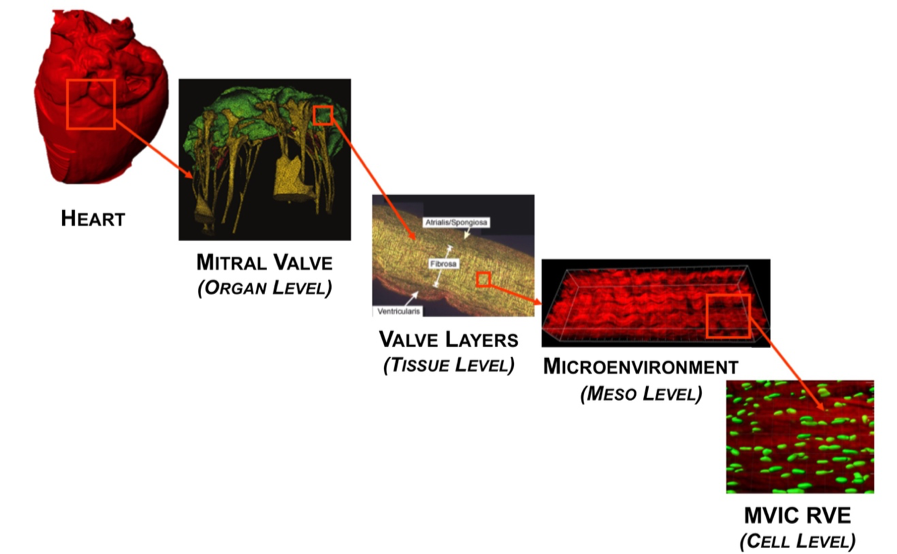
\includegraphics[width=\textwidth]{Images/chapter1/multiscalevalve.png}
\caption{The multiscale nature of heart valve biomechanics: a representation of the mitral valve at the organ-, tissue-, and cell-levels. At the tissue-level: a circumferentially oriented cross-section of the mitral valve anterior leaflet stained with Movat pentachrome, which colors collagen yellow, elastic fibers black, and hydrated PGs and GAGs blue. At the cell-level: a transmission electron micrograph of a mitral VIC from the fibrosa layer. \cite{salma_heart_2016}}
\label{fig:multiscalevalve}
\end{figure}
%-------------------	 end FIGURE 	-------------------%


%-------------------	begin FIGURE 	-------------------%
\begin{figure}
\centering
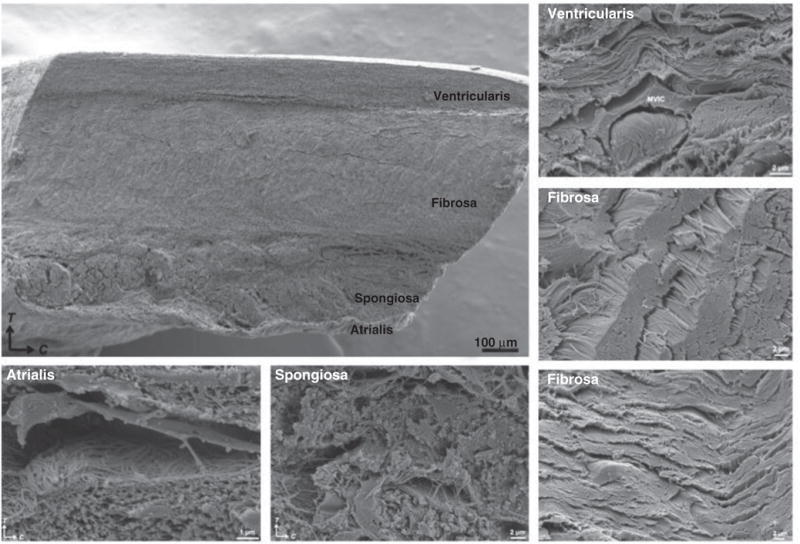
\includegraphics[width=\textwidth]{Images/chapter1/valvelayers.jpg}
\caption{Scanning electron micrograph of the multilayered microenvironment of the MV anterior leaflet. Individual micrographs of each layer are also presented: elastin-rich ventricularis and atrialis, highly collagenous fibrosa, and proteoglycan-rich spongiosa. The collagen fibrils and elastic fibers closely surround the interstitial cells and highlight the long cellular extensions. In the fibrosa, collagen fibrils are aligned in the circumferential direction of the leaflet, which is responsible for the observed anisotropy in leaflet mechanical behavior. (T: transmural, C: circumferential). \cite{salma_heart_2016}}
\label{fig:valvelayers}
\end{figure}
%-------------------	 end FIGURE 	-------------------%




\subsection{Biomechanical function of heart valves}

It has been demonstrated that the individual layers of the aortic valve are not only vastly different in their structure, but also in their mechanical behavior. Two key studies have investigated individual layer behavior of the AV leaflet. Vesely et al. observed the extensibility of intact tissue under uni-axial tension to be significantly different from the individual layer responses [71]. Stella et al. also observed measurably different behaviors under bi-axial loading of separated layers, and reported the intact tissue response to be intermediate to the separated responses [72]. Due to these consistently observed differences in layer behavior, examining the leaflet in an intact state is far more physiologically relevant. 


\section{Valvular diseases and prevalence}

    Cardiovascular diseases are the number one killer in the United States and around the world. Heart valve treatment is a common cardiovascular surgical procedure with over 100,800 done annually in the U.S. alone \cite{mozaffarian_heart_2016} and 275,000 to 370,000 in developed nations \cite{manji_future_2012}. Calcification is the primary cause of AV failure and currently there exists no proven therapy for halting this progression. Calcified aortic valve disease is a slow, progressive, multi-factorial disorder that is more common with age, without being an inevitable consequence of aging \cite{towler_molecular_2013,freeman_management_2002,freeman_spectrum_2005,kurtz_aortic_2010,beckmann_insights_2010}. The disease is characterized by a thickening and calcification of the leaflets and is diagnosed in two stages: aortic sclerosis and aortic stenosis. aortic sclerosis, present in more than 25\% of patients over the age of 65 \cite{obrien_pathogenesis_2006}, represents the early onset of calcified aortic valve disease absent of physical obstruction to the left ventricular outflow. Aortic stenosis exists in 2-5\% of the elderly population \cite{obrien_pathogenesis_2006} is characterized by late stage obstruction and associated with impaired leaflet motion, valve tissue adaptation, and resistance to blood flow \cite{poggio_noggin_2013,grau_analysis_2012,gharacholou_aortic_2011,pflederer_aortic_2010} . Although aortic sclerosis causes significant thickening of the AV leaflets, there is little to no change in the mechanical properties of the valve, making the disease relatively asymptomatic. Recent statistics have shown that within 10 years of their initial diagnosis, 10\% of aortic sclerotic patients reach a state of severe calcified aortic valve disease that requires immediate AV replacement once symptoms emerge \cite{gharacholou_aortic_2011}. 
    
    
    Aortic stenosis has been identified as the end-stage of calcified aortic valve disease that progresses from the microscopic early changes of aortic sclerosis to, in a subset of patients, asymptomatic and then symptomatic Aortic stenosis \cite{kurtz_aortic_2010,otto_calcific_2010,aikawa_look_2012}. Once aortic sclerosis is detected, there is an increased risk of cardiovascular events. In early Aortic stenosis, when mild symptoms begin to present, survival rates deviate much more than expected and decline dramatically with the onset of severe symptomatic Aortic stenosis. Over the last decade, several clinical trials, mostly extensions of atherosclerosis-related studies, have been performed to halt the progression of calcified aortic valve disease with randomized studies showing substantial equivalence between treatments and placebo \cite{parolari_do_2011,moura_rosuvastatin_2007,cowell_randomized_2005,benton_statins_2009,rossebo_intensive_2008}. However, there are currently no pharmacological therapies available to treat calcified aortic valve disease symptomatic patients that are considered superior to full valve replacement surgery. 




\subsection{Bioprosthetic heart valve replacements}
     
    Since initially introduced in 1960, valve replacement surgery has significantly reduced the mortality of patients with heart valve diseases \cite{braunwald_complete_1960,pibarot_valvular_2009,ross_replacement_1967}. As reported by The Society of Thoracic Surgeons 59,555 Americans underwent valve replacement surgery in 2014 (48,060 AV replacement, 9595 MV replacement, 1900 replacing both the AV and MV).  Of the four heart valves, the AV has been studied most, followed next by the MV, whereas fewer studies have been performed. This is primarily due to the fact that the AV \cite{christie_age_1995,merryman_correlation_2006,adamczyk_characteristics_2002,sacks_aortic_1998,billiar_biaxial_2000,billiar_biaxial_2000b,vesely_comparison_1998,vesely_micromechanics_1992,vesely_role_1998} and MV \cite{stella_biaxial_2007,sacks_surface_2002,gorman_dynamic_1996,gorman_effect_2004} are more suspectible to diseases and more frequently warrant replacement surgery. While important differences exist in valve geometries and function, the mechanics of the AV are primarily used as a baseline for the development of models of heart valve function. Thus, this dissertation will focus on the aortic valve as an example as it is one of the most common valves for heart valve replacement surgeries. The same framework proposed in this dissertation is otherwise applicable to the mitral and other valves. 
    
    
    Current clinically surgical valve replacement utilize either mechanical valves (usually made of pyrolytic carbon or titanium) or valves constructed from biologically\Hyphdash derived soft tissues.  Mechanical valves have evolved significantly since the first ball-and cage design, spanning a variety of shapes sizes and materials and rarely experiencing mechanical failure. However, they non-physiologic blood flow patterns and results in a substantial thrombogenic response, requiring lifelong post-operative anticoagulation therapy and its inherent risks \cite{pibarot_valvular_2009}.
    
    
    On the other hand, bioprosthetic heart valves (BHVs) are comprised of decellularized bovine pericardium or porcine aortic valve tissues (most commonly the pericardium) and offer a higher degree of functionality including improved hemodynamics and a higher resistance to thrombosis. Although they are chemically fixed, these tissues are still prone to valve calcification, structural deterioration, and eventual failure \cite{sacks_collagen_2002,vyavahare_mechanisms_1999}. Durability is the major limitation of current BHV technology—the 15-year durability of heterograft BHVs in the aortic position is less than 50\% for middle-aged patients and slightly better for older patients, however BHVs continue to be the preferred replacement valve \cite{siddiqui_bioprosthetic_2009}. Regardless of its shortcomings, heart valve replacement has had a substantial impact on cardiac surgery with a consistently increasing number of surgeries per year \cite{starr_artificial_2007}.

    
    Currently, bovine pericardium (BP) and porcine AV tissues are still the only clinically approved xenograft biomaterial for BHVs. Other tissue sources have been pursued, but none has reached clinical widespread application. Collagenous soft tissues used for bioprosthetic devices are EXL, often using glutaraldehyde (GLUT), to suppress antigenic properties of the tissue and to stablized the CFA \cite{khor_methods_1997}. GLUT is popular due to its affordability and solubility in an aqueous solution \cite{jayakrishnan_glutaraldehyde_1996}. However, GLUT is also implicated in the calcification of BHVs \cite{golomb_role_1987}, which is further accelerated by mechanical stress \cite{schoen_calcification_2005}. There exists some alcohol based pretreatments for GLUT EXL BHV to reduce calcification \cite{vyavahare_prevention_1997}, but there is little that we understand about the mechanical properties of EXL tissue. Specifically, there have been no attempt to constitutively model exogenous cross-linking and how it modulate the stresses. 
    
    
    GLUT is observed to significally stiffen the ECM but not that of the collagen fibers \cite{gentleman_mechanical_2003,yang_mechanical_2008,yang_micromechanical_2007}. It is also a Schiff-base, which means it reversibly reacts with aldehydes. Over time, this scission-healing behavior allows for a gradual change in the reference state, resulting in PS. This has yet to be properly modeled in biological tissues. Although there have not been any introduction of new cross-linking methods from a industrial stand point, research in alternative technologies such as carbodiimide is ongoing \cite{sung_crosslinking_2003,billiar_effects_2001,kemp_effects_1995}, including a new method developed by our collaborator to stablized elastin and GAGs in addition to collagen \cite{tam_novel_2015}. As GLUT and these other exogenous cross-linking methods remain necessary, it is important that we understand their role in predicting the fatigue and durability of bioprothetic devices.
    
    
    The most recent development in BHV technology is the percutaneous (or transcatheter) valve replacement. This technology is a minimally invasive procedure which delivers the replacement valves with catheterization from a large blood vessel, most commonly the femoral artery. This procedure makes valve replacement more feasible for those who cannot tolerate full surgical interventions. However, this new technology also presents additional design challenges, including complex folding and compression during delivery. As a result, the leaflets are required to be significantly thinner than in traditional BHVs, which increases the leaflet stress and potentially the rate of failure. Existing data on transcatheter aortic valve interventions suggest a 2-year mortality rate of 33.9\% overall \cite{mozaffarian_heart_2016} and over 68\% when specifically replacing stenotic aortic valves \cite{makkar_transcatheter_2012}. As such, this further accentuates the need to develop an approach to improve BHV durability. 
    
    
    BHVs have become the preferred replacement valve. The sustained growth of AV and MV replacement surgeries, the lack of substantial technological breakthroughs in the field over the last decades \cite{soares_biomechanical_2016}, and the continuous need to improve BHV durability, promote a strong necessity to develop a higher understanding of the mechanisms involved in BHV function and failure.  Critical BHV engineering aims to ensure valve functionality for its clinical performance with a combination of hemodynamic, biomechanical and biological aspects, and to predict and extend as much as possible valve durability. The major hurdle of the technology remains the lifespan of the BHV implant. Improvements to BHV design and durability have substantial clinical impact, even if marginally (i.e. 3–5 years) \cite{jamieson_carpentier_1998}.
    

\section{Mechanisms of Bioprosthetic heart valve fatigue and failure}

    The mechanisms of limiting the durability of BHV can be divided into two categories: mineralization and Mechanical fatigue \cite{schoen_tissue_1999,schoen_pathology_2001,schoen_calcification_2005}. Tissue calcification primarily initiates from devitalized residual cells, usually from glutaraldehyde pretreatment \cite{schoen_calcification_2005}. Mineralization occurs due to interactions between the cell membrane phosphates and the calcium within the extracellular fluids. Mechanical stress appears to accelerate calcification, but mineralization and also occur in the absence of mechanical stress. 
    To some extent, mineralization and calcification are interdependent processes \cite{sacks_collagen_2002}. Evidence suggests that mechanical deformation, either dynamic or static, potentiates mineralization but the mechanisms are unclear \cite{schoen_tissue_1999}. High levels of calcification have been generally reported to coincide with regions of high flexure, especially the commissures and basal attachment margin \cite{thubrikar_aortic_1990,schoen_pathology_2001}. It is postulated that disruption of the collagen structure may produce new nucleation sites for calcific crystals, promoting mineral growth, or simply allow fluid insudation leading to exposure to greater amounts of calcium and phosphorus ions \cite{schoen_tissue_1999}. Conversely, mechanical damage could result from direct fatigue effects, stress concentrations within the cusp induced by calcification or direct structural damage induced by calcification \cite{schoen_calcification_2005}. Many BHVs fail with little or no calcification \cite{schoen_tissue_1999,schoen_anatomic_1985,schoen_pathology_2001}. In the study by Sacks and Schoen, it was observed that regions with disruptions in collagen fiber architecture did not necessarily correspond with regions with high calcification (Fig. \ref{c1:fig:calcificationdamage}) \cite{sacks_collagen_2002}. Thus, calcification independent could be equally important mechanisms for BHV failure.
    
%-------------------	begin FIGURE 	-------------------%
\begin{figure}
\centering
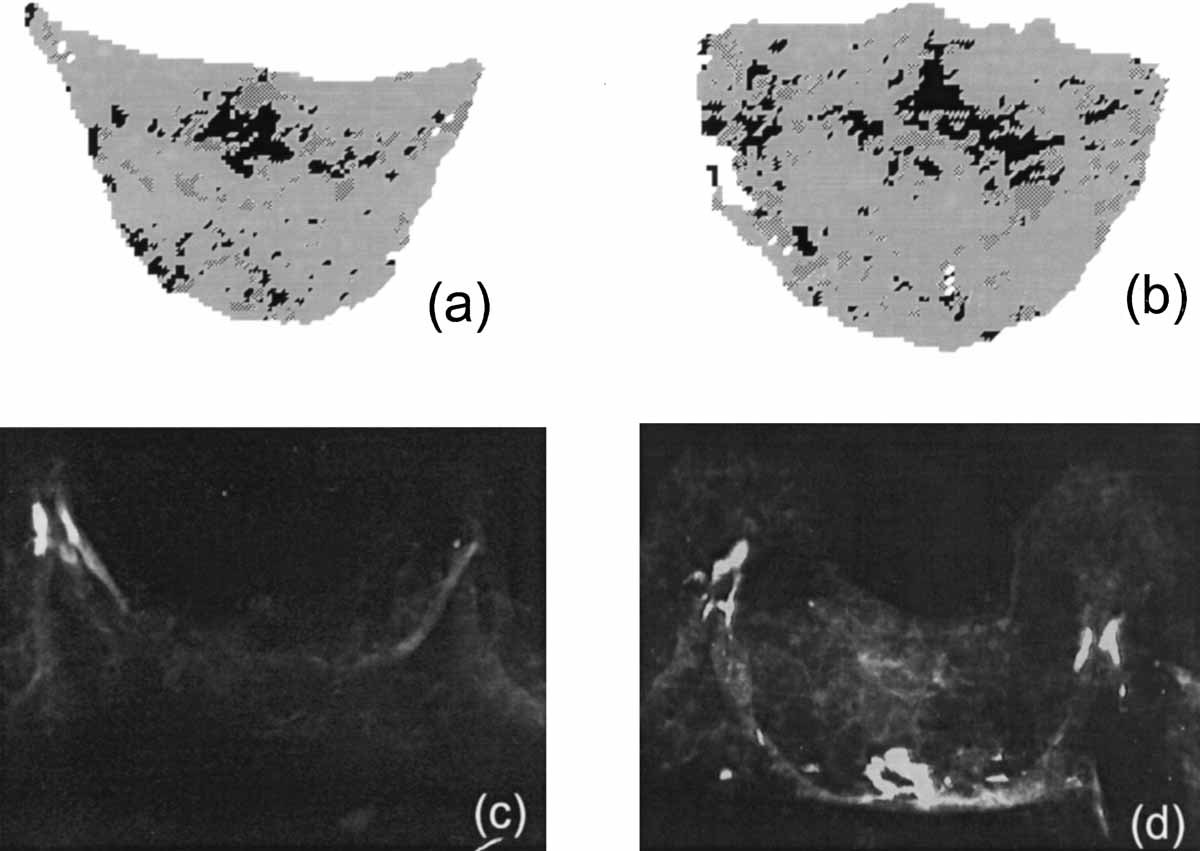
\includegraphics[width=5.0in]{Images/chapter1/calcificationdamage.jpg}
\caption{(a,b) Regions of collagen fiber damage derived from SALS data by plotting regions with large distruptions in collagen fiber structure in black. (c,d) Corresponding X‐ray photos showing pronounced calcification along the commissure and basal attachment. In both cusps regions of structural damage did not spatially correlate with regions of calcification. As shown in (e), this lack of correlation was consistent in all explanted cusps. (Adapted from \cite{sacks_collagen_2002})}
\label{c1:fig:calcificationdamage}
\end{figure}
%-------------------	 end FIGURE 	-------------------%



    Damage initially accumulates in the collagen fiber architecture (CFA) (Fig. \ref{c1:fig:damageprocess}) which in turn lead to tearing and delamination \cite{vyavahare_mechanisms_1999}. Predicting tearing and delamination (fracturing) is an extremely complex process even for solid materials without biological factors. Before tackling this, a solid groundwork for the processes that lead to this failure is needed. For BHVs this can be done by predicting the accumulation of collagen fiber damage, which leads to the development of micro-tears in the extracellular matrix (ECM) before propagating to full tissue-scale tearing. Thus, simulating fiber-level damage can be used to form preliminary estimation of BHV durability. 

\begin{figure}[hbt]
\centering
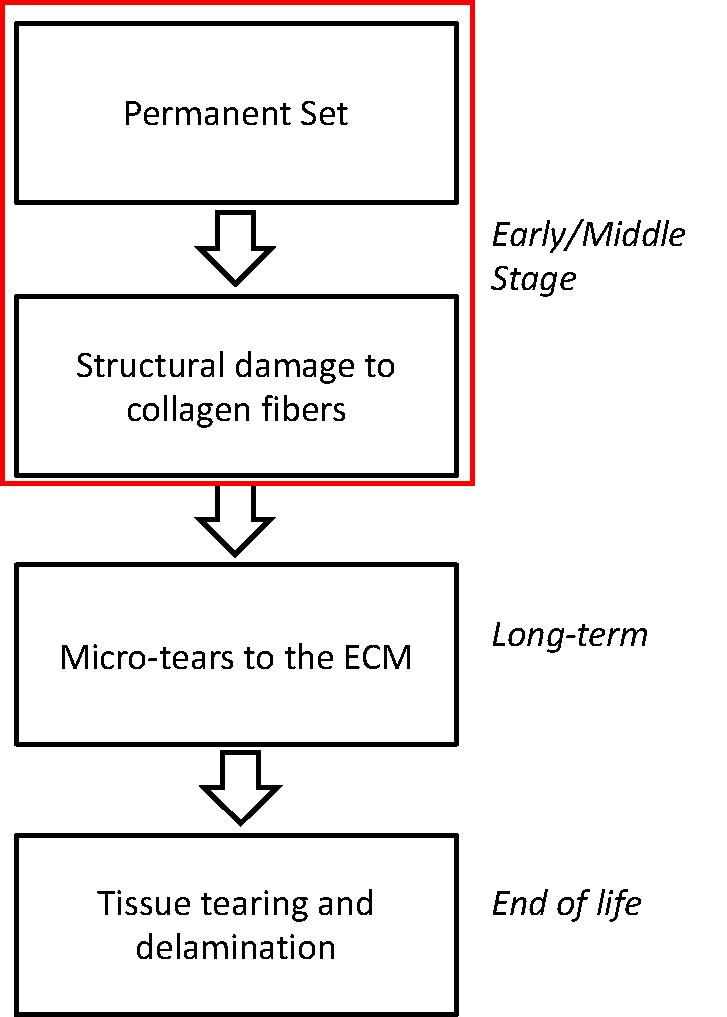
\includegraphics[width=2.75in]{Images/chapter1/damageprocess.pdf}
\caption{Stages of fatigue and failure. We will focus on the early and mid-term (Red).}
\label{c1:fig:damageprocess}
\end{figure}

    The most significant change in response to cyclic loading is the change in geometry of the BHV leaflets. In a study on the porcine aortic BHVs \cite{smith_high_1997},  Smith \textit{et al}. found significant changes in the unloaded geometry of BHVs after AWT, especially in the belly region of the leaflets (Fig. \ref{c1:fig:PSeffects}A). By changing the unloaded reference configuration, the shape of the leaflets and their mechanical response will change as well. The further analysis has shown that significant structural damage occurred within the belly region as compared to other regions of the leaflet, where the stress significantly increased \cite{smith_fatigue_1999}. Interestingly, Smith et al. also found most the most significant changes in BHV leaflet geometry to occur within first 50 million cycles \cite{smith_high_1997}. Moreover, Sacks and Smith \cite{sacks_effects_1998} also found that there was minimal structural damage in this early stage (Fig. \ref{c1:fig:PSeffects}B). This is further supported by another study by Wells \textit{et al} \cite{wells_cyclic_2005}, where they found minimal structural changes during the first 50 million cycles for the pressure fixed BHVs, with most significant change observed in the first million cycles. Clearly, there is a non-damage based mechanism at play that changes the geometry of the material, with significant impact on the early stage of cycling and the rate of fatigue in later stages. 


\begin{figure}[hbt]
\centering
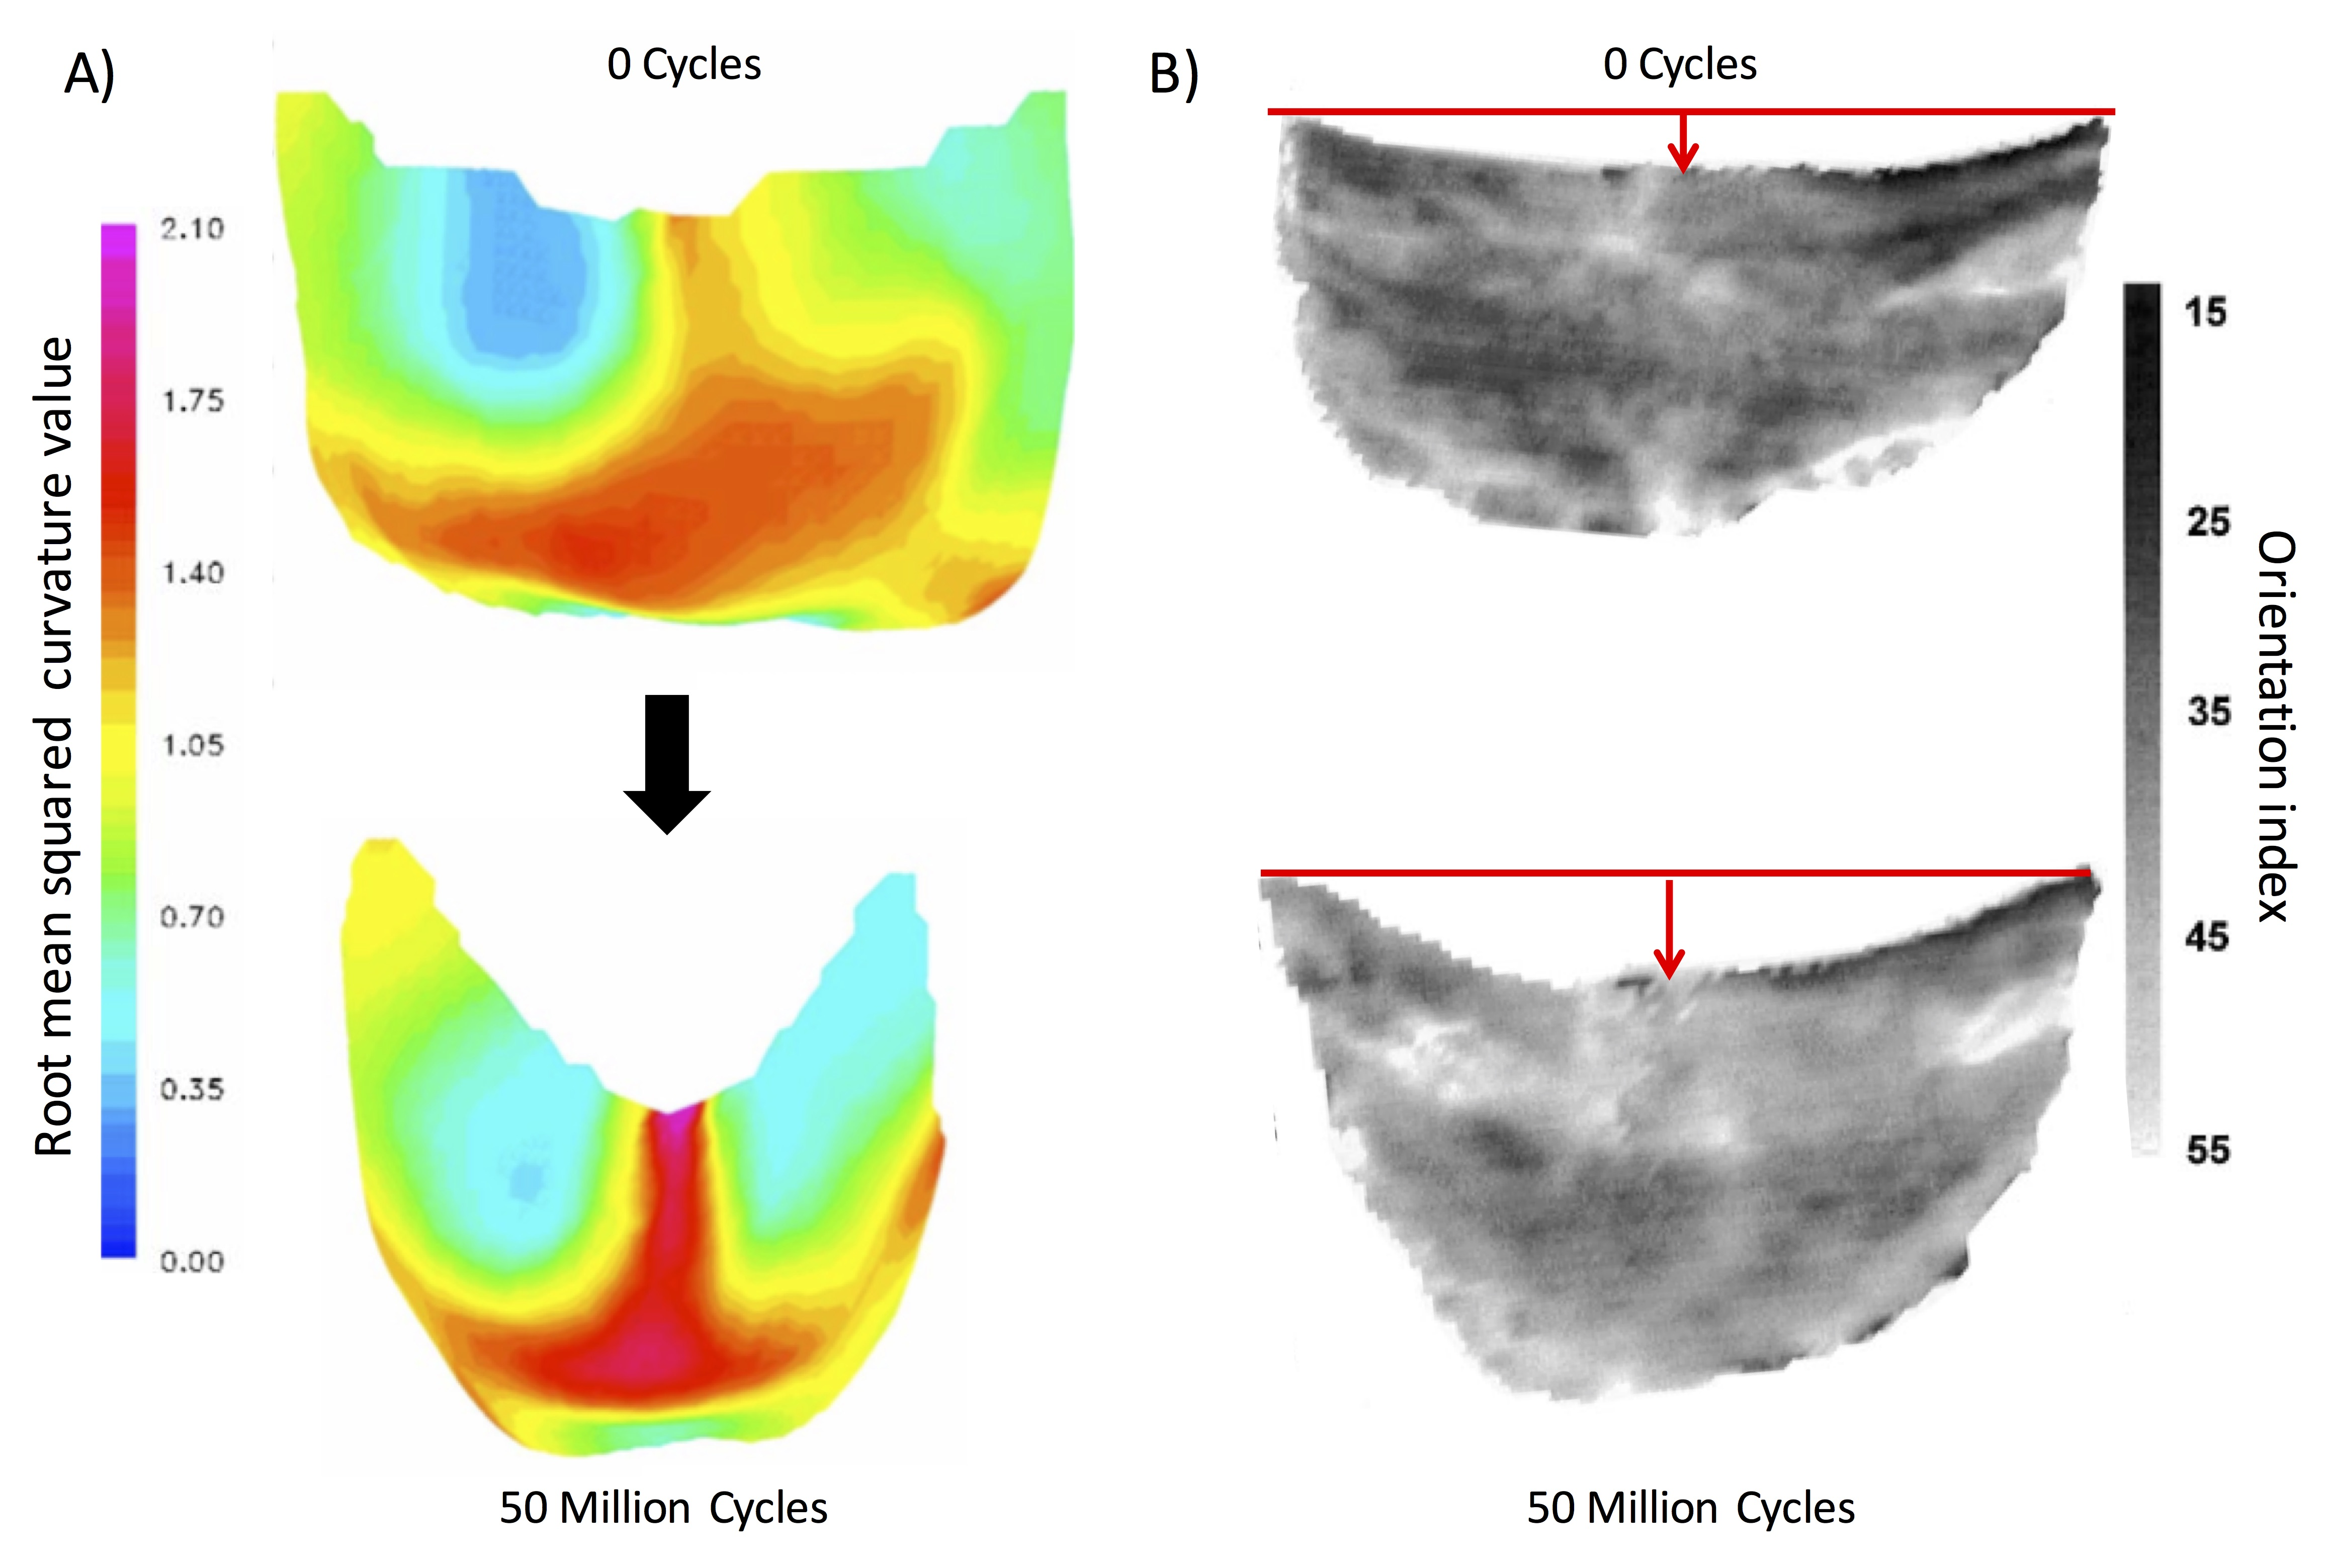
\includegraphics[width=\textwidth]{Images/chapter4/figure1}
\caption{A) The 3D unloaded geometry a BHV leaflet before and after cyclic loading, with the color indicating the local root mean squared curvature. The most significant change in geometry is in the belly region. B) BHV leaflet collagen fiber architecture, showing that the collagen fiber architecture are convected by the dimensional changes. The grayscale scale bar shows the orientation index (OI), which is angle containing 50 \% of fibers. The lack of changes in the OI suggests that minimal damage to the collagen fiber architecture has occurred.}
\label{c1:fig:PSeffects}
\end{figure}



    


    Soft-tissue-derived exogenously cross-linked (EXL) biomaterials continue to play an important role in surgical repair and medical devices. This is especially true for bioprosthetic heart valves (BHV), by having advantages in immunogenic and mechanical behaviors [1]. Despite ongoing research, our understanding of these materials and of the mechanisms leading to their failure remains at an empirical level. The need for advancements in predicting the material behavior is further underscored by the development of percutaneously-delivered BHV devices. While these devices reduce surgical risk, they also present additional challenges for the design of the BHVs due to limitations in thickness, and folding and compression during delivery. A significant challenge prohibiting accurate and predictive simulations of BHVs are a lack of understanding of the effect of exogenous cross-linkers, such as glutaraldehyde (GLUT), and an associated predictive material model in response to cyclic loading. GLUT EXLs form polymeric chains through the cross-linking process which more tightly bond the collagen fibers to the non-fibrous matrix, increasing the non-fibrous matrix stiffness and fiber-fiber interactions. However, GLUT EXLs also undergo Schiff-base reactions that are hypothesized to lead to scission-healing behaviors that result in the permanent set (PS) phenomena. PS continuously changes in the reference geometry of the BHV and can induce extra-physiological stress concentrations in the BHV leaflets. Microstructural-based constitutive models for tissues and their use in valve-level simulations can lead to insights into the underlying mechanisms and more accurate prediction of their long-term performance. Thus, we seek to develop a framework for modeling and simulating biologically-derived EXL soft collagenous tissues for BHV, accounting for the effects of EXL, PS, and collagen fiber-level damage, taking the following approach:


    \subsubsection*{Specific Aim 1: Establish and validate a generalized nonlinear hyperelastic meso-scale structural constitutive model (MSSCM) for native collagenous soft tissues.} As a first step towards modeling EXL biomaterials, we will take a generalized meso-scale (at the level of the constituent fibers) structural modeling approach to accurately model the mechanical response of soft tissues. Firstly, we will develop an improved analytical method for processing extant mechanical data under generalized 2D deformations, to more accurately characterize the tissue. Next, after posing the model form, we will extensively validate critical assumptions such as affine fiber deformation, mechanical response of the constituent fibers, and direct integration of physical measurements of the fiber microstructure. The validation will be done through extensive mechanical characterization through different testing methods and microstructural characterization at the 1) micro-scale (fibril) and 2) meso-scale using optical techniques such as multiphoton microscopy and x-ray scattering. The two tissues we will examine for application and validation of the model are the ovine pulmonary artery and the porcine mitral valve leaflets, which offer a diverse selection structural composition to span applicable realms.
    
    \addcontentsline{toc}{subsubsection}{Specific Aim 1: Establish and validate a generalized nonlinear hyperelastic meso-scale structural constitutive model for native collagenous soft tissues.}%


    \subsubsection*{Specific Aim 2: Extend the MSSCM to account for of the presence of EXLs and subsequent response to continuous cyclic loading.} Using GLUT treated bovine pericardium, we aim to separately model the mechanical response of the collagen fibers, matrix, and fiber-fiber interactions due to cross-linking. For this, we will develop a method to map the collagen fiber architecture characterized from the native state to the EXL state. Next, we will develop a PS model based on a constantly evolving referential configuration that occurs due to scission-healing when the tissue is held in an extended state. We will validate the model for orientation and strain level dependence. The model will be tested and validated using constant cyclic strain, as well as stress control experimental data. Finally, we will extend the model for collagen fiber-level damage that may occur during cyclic loading. 
    
    \addcontentsline{toc}{subsubsection}{Specific Aim 2: Extend the meso-scale structural constitutive model to account for of the presence of EXLs and subsequent response to continuous cyclic loading.}%
    
    
    \subsubsection*{Specific Aim 3: Application to organ/device level}. In this final aim, we will develop a full 3D finite element implementation utilizing the open source FEniCS framework for greater modularity and extensibility. The model will utilize real BHV geometries and fiber microstructure mapped from experimental measurements, and will be validated by simulating of the PS experiments from SA 2. We will further perform organ-level study of PS and collagen fiber-level damage using accelerated wear testing of specialized ovine mitral transcutaneous BHVs. We will use an inverse modeling approach with micro-CT measurements [2] to quantify changes in mechanical behaviors. The validated model and rate constants will then be used to parametrically examine the changes in BHV geometry and stress distribution overtime, where change in resting and loaded geometry of the valve as well as the development of stress concentrations are the early indicators of BHV failure. We will also explore initial geometries and material properties which may minimize the risks of these effects. With this, we aim to develop a better understanding of the underlying process that occurs during long-term cyclic loading using our constitutive modeling approach and device level applications, and translate the insights gained to improving BHV design and durability. 

    \addcontentsline{toc}{subsubsection}{Specific Aim 3: Application to organ/device level}%

\section{Motivation, innovation, and specific aims}

\subsection{Motivation and innovation}

\subsubsection{The Lack of Established Constitutive Models for Planar Soft Tissues}
    Although finite element analysis is an effective method for stress analysis, truly predictable computational simulations cannot be done without an accurate constitutative model for the underlying biomechanical response. There is currently a lack of a well establish constitutive model for collagenous soft tissues. Currently each research group uses their own model, often simple forms of the Fung model or linear functions of the invariants. These models are often not informative, offering no insights into the structural functional relationship. Unfortunately, this also means these models are also lack predictive capabilities as a result, and can only interpolated the experimental data. This is a problem for simulating the effect of fatigue in which the geometry and the mechanical properties of BHVs can change significantly, necessating extrapolation of the data into unmeasured regime. Structural models theories exists [27-29] but is under utilized and not well validated for the wide range of tissue that may be applicable for BHV devices. Thus, the establishment of a generalized and well-validated constitutive model is a critical step the in process of developing accurate simulations of BHV devices.

\subsubsection{The Lack of Fundamental Modeling Approach for EXLs, PS, and Collagen Fiber-Level Damage in Soft Tissue-Derived Biomaterials}

    There is no accepted constitutive model for the effect of EXLs on the mechanical properties of soft tissues. Without understanding the mechanical properties of the subcomponents of the bioprosthetic biomaterial, we cannot properly predict how they will change over time. Although calcification plays an important role in the failure of BHVs, addressing this concern alone will not alleviate the loss of functional due to mechanical fatigue. Although this proposal will not simulate the full process to failure, as previously indicated (1.B), we will for the first time examine the early stages of fatigue in PS and collagen fiber-level damage. This will nevertheless give us a firsthand estimate of BHV durability and design, as well as build the foundation for future extensions of the model.

\subsubsection{The Lack of A Framework for Simulating The Response of BHV Devices in Response to Cyclic Loading}

    Our ability to evaluate the design of BHVs devices are directly linked to our ability to understand and rigorously experiment on the in vivo durability of these devices. However, clinical and large anime testing remains costly and reserved for latter stages of the design analysis. Furthermore, it is difficult for such studies to paint a complete picture of the underlying mechanisms due bio-variability and direct ways of controlling the biological system. This has led to a stagnation of BHV device development \cite{schoen_cardiac_2005}. Computational simulations can be an exceptional complement to in vitro and animal experiment in understanding how biomechanical properties evolve and drive mechanical function and performance. Indeed, the consensus in the field is the increasing role of computational simulation in the development of cardiovascular devices [30]. Finite element analysis is unknown for its ability to determine the stress at a device-level and can be used to reiterate on conceptual designs to optimize the functional properties of prototypes [31-33]. Thus, computational implementation of the tissue structural PS-fatigue model is the best way to guide our understanding of BHV device performance.

\subsection{Specific aims}
    Soft-tissue-derived exogenously cross-linked (EXL) biomaterials continue to play an important role in surgical repair and medical devices. This is especially true for bioprosthetic heart valves (BHV), by having advantages in immunogenic and mechanical behaviors [1]. Despite ongoing research, our understanding of these materials and of the mechanisms leading to their failure remains at an empirical level. The need for advancements in predicting the material behavior is further underscored by the development of percutaneously-delivered BHV devices. While these devices reduce surgical risk, they also present additional challenges for the design of the BHVs due to limitations in thickness, and folding and compression during delivery. A significant challenge prohibiting accurate and predictive simulations of BHVs are a lack of understanding of the effect of exogenous cross-linkers, such as glutaraldehyde (GLUT), and an associated predictive material model in response to cyclic loading. GLUT EXLs form polymeric chains through the cross-linking process which more tightly bond the collagen fibers to the non-fibrous matrix, increasing the non-fibrous matrix stiffness and fiber-fiber interactions. However, GLUT EXLs also undergo Schiff-base reactions that are hypothesized to lead to scission-healing behaviors that result in the permanent set (PS) phenomena. PS continuously changes in the reference geometry of the BHV and can induce extra-physiological stress concentrations in the BHV leaflets. Microstructural-based constitutive models for tissues and their use in valve-level simulations can lead to insights into the underlying mechanisms and more accurate prediction of their long-term performance. Thus, we seek to develop a framework for modeling and simulating biologically-derived EXL soft collagenous tissues for BHV, accounting for the effects of EXL, PS, and collagen fiber-level damage, taking the following approach:


    \subsubsection*{Specific Aim 1: Establish and validate a generalized nonlinear hyperelastic meso-scale structural constitutive model (MSSCM) for native collagenous soft tissues.} As a first step towards modeling EXL biomaterials, we will take a generalized meso-scale (at the level of the constituent fibers) structural modeling approach to accurately model the mechanical response of soft tissues. Firstly, we will develop an improved analytical method for processing extant mechanical data under generalized 2D deformations, to more accurately characterize the tissue. Next, after posing the model form, we will extensively validate critical assumptions such as affine fiber deformation, mechanical response of the constituent fibers, and direct integration of physical measurements of the fiber microstructure. The validation will be done through extensive mechanical characterization through different testing methods and microstructural characterization at the 1) micro-scale (fibril) and 2) meso-scale using optical techniques such as multiphoton microscopy and x-ray scattering. The two tissues we will examine for application and validation of the model are the ovine pulmonary artery and the porcine mitral valve leaflets, which offer a diverse selection structural composition to span applicable realms.
    
    \addcontentsline{toc}{subsubsection}{Specific Aim 1: Establish and validate a generalized nonlinear hyperelastic meso-scale structural constitutive model for native collagenous soft tissues.}%


    \subsubsection*{Specific Aim 2: Extend the MSSCM to account for of the presence of EXLs and subsequent response to continuous cyclic loading.} Using GLUT treated bovine pericardium, we aim to separately model the mechanical response of the collagen fibers, matrix, and fiber-fiber interactions due to cross-linking. For this, we will develop a method to map the collagen fiber architecture characterized from the native state to the EXL state. Next, we will develop a PS model based on a constantly evolving referential configuration that occurs due to scission-healing when the tissue is held in an extended state. We will validate the model for orientation and strain level dependence. The model will be tested and validated using constant cyclic strain, as well as stress control experimental data. Finally, we will extend the model for collagen fiber-level damage that may occur during cyclic loading. 
    
    \addcontentsline{toc}{subsubsection}{Specific Aim 2: Extend the meso-scale structural constitutive model to account for of the presence of EXLs and subsequent response to continuous cyclic loading.}%
    
    
    \subsubsection*{Specific Aim 3: Application to organ/device level.} In this final aim, we will develop a full 3D finite element implementation utilizing the open source FEniCS framework for greater modularity and extensibility. The model will utilize real BHV geometries and fiber microstructure mapped from experimental measurements, and will be validated by simulating of the PS experiments from SA 2. We will further perform organ-level study of PS and collagen fiber-level damage using accelerated wear testing of specialized ovine mitral transcutaneous BHVs. We will use an inverse modeling approach with micro-CT measurements [2] to quantify changes in mechanical behaviors. The validated model and rate constants will then be used to parametrically examine the changes in BHV geometry and stress distribution overtime, where change in resting and loaded geometry of the valve as well as the development of stress concentrations are the early indicators of BHV failure. We will also explore initial geometries and material properties which may minimize the risks of these effects. With this, we aim to develop a better understanding of the underlying process that occurs during long-term cyclic loading using our constitutive modeling approach and device level applications, and translate the insights gained to improving BHV design and durability. 

    \addcontentsline{toc}{subsubsection}{Specific Aim 3: Application to organ/device level}%


\newpage

\bibliographystyle{plainnat}
\bibliography{phd}



